\documentclass[letterpaper]{article}
\author{Jonathan Chan (15354146)}
\title{PHYS 319\\Labs 5 and 6 Notes}

\usepackage{fullpage}
\usepackage{minted}
\usepackage{siunitx}
\usepackage{hyperref}
\usepackage{graphicx}

\begin{document}
	\maketitle
	
	The goal of this lab is to measure distances with the ultrasonic ranger. References to specific values and other documentation notes refer to \url{http://www.robot-electronics.co.uk/htm/srf04tech.htm}. The steps to achieve this can be outlined as follows:
		\begin{enumerate}
			\item Send a trigger pulse to the ranger. According to the documentation, this pulse needs to be $\SI{10}{\micro s}$ long.
			\item Wait for the echo input to be raised. This can be done by setting a low-to-high interrupt on the echo pin.
			\item Time the length of the echo pulse sent by the ranger. We will set \texttt{TAR} to 0 and retrieve the value of \texttt{TAR} when the echo pin is lowered, which can be done by setting a high-to-low interrupt on the echo pin. We will use the SMCLK timer, which runs at $\SI{1}{M\hertz}$, meaning that the maximum length that can be measured without overflowing is $\SI{65 535}{\micro s}$. However, according to the documentation, the ranger will time out and lower the echo pin after $\SI{30 000}{\micro s}$, so we aren't in danger of overflowing. 
			\item Convert the measurement to distance in centimetres. According to the documentation, we need to divide by $58$. Since we're limited to sending one byte at a time, we can also set the value to $0$ if the distance exceeds $\SI{255}{cm}$ to prevent the plot from graphing meaningless overflowed values.
			\item Send the data to the Python plot. This portion of the code will come from the provided temperature measurement program.
			\item Repeat the measurement. According to the documentation, we need to wait $\SI{10}{ms}$ to allow the ranger to recharge. I've set the delay to $\SI{100}{ms}$ to smooth out the data and prevent rapid changes in the position of the ranger from being recorded.
		\end{enumerate}
	With some measurements using a metre stick, the distances measured by the ranger are indeed accurate to the centimetre. It also appears that it cannot measure anything closer than $\SI{3}{cm}$. Of course, we are also upper-bounded at $\SI{255}{cm}$ by the size of one byte, even if the limit of the ranger itself is $\SI{30 000}{\micro s} / \SI{58}{\micro s*cm^{-1}} \approx \SI{517}{cm}$. We can circumvent this by dividing the the value by $2$ in the C program then multiplying it by $2$ again in the Python program, so that the maximum measurable distance is $\SI{510}{cm}$, at the cost of decreasing the precision to a granularity of $\SI{2}{cm}$.
	
	Below is the modified \texttt{main.c} file, with the remaining files unchanged from \url{http://www.phas.ubc.ca/~michal/phys319/temperature_demo4.zip}. Of course, the axis ranges and labels of the plot should be adjusted accordingly. After the C program has been written to the microprocessor, connect P1.4 to the ranger's trigger pin, connect P1.6 to the ranger's echo pin through a $\SI{1}{k\ohm}$ resistor, connect the ranger to $\SI{5}{V}$ and ground, connect the microprocessor to ground, and run \texttt{python python-serial-plot.py}.
	
	\newpage	
	\noindent \textit{\texttt{main.c}}:
	\begin{minted}{c}
    #include "msp430.h"
    #define   TXD       BIT2
    #define   RXD       BIT1
    #define   TRIG      BIT4
    #define   ECHO      BIT6
    #define   CM        58
    
    unsigned int TXByte;
    void main(void) {
        WDTCTL    = WDTPW + WDTHOLD;  // Stop WDT
    
        BCSCTL1   = CALBC1_1MHZ;      // Set range
        DCOCTL    = CALDCO_1MHZ;
        BCSCTL2  &= ~(DIVS_3);        // SMCLK = DCO = 1 MHz
        P1SEL     = BIT1 + BIT2;      // P1.1 = RXD, P1.2=TXD
        P1SEL2    = BIT1 + BIT2;      // P1.1 = RXD, P1.2=TXD
        UCA0CTL1 |= UCSSEL_2;         // Use SMCLK
        UCA0BR0   = 104;              // Set baud rate to 9600 with 1MHz clock (Data Sheet 15.3.13)
        UCA0BR1   = 0;                // Set baud rate to 9600 with 1MHz clock
        UCA0MCTL  = UCBRS0;           // Modulation UCBRSx = 1
        UCA0CTL1 &= ~UCSWRST;         // Initialize USCI state machine
    
        P1DIR    |= TXD;
        P1OUT    |= TXD;
        P1DIR    |=  TRIG;            // set trigger output
        P1DIR    &= ~ECHO;            // set echo input
        P1IE     |=  ECHO;            // use echo input as interrupt
        TACTL     = TACLR;            // reset clock
        TACTL     = TASSEL_2 | MC_2;  // set SMCLK timer to count up at 1 MHz
        __enable_interrupt();
    
        while (1) {
            P1OUT |=  TRIG;                     // start trigger signal
            __delay_cycles(10);                 // we need a >10 us pulse and one clock cycle is 1 us
            P1OUT &= ~TRIG;                     // end trigger signal
    
            P1IES &= ~ECHO;                     // interrupt on low to high
            __bis_SR_register(LPM0_bits + GIE);
            TAR = 0;
            P1IES |=  ECHO;                     // interrupt on high to low
            __bis_SR_register(LPM0_bits + GIE);
    
            TXByte = TAR / CM;                  // distance in cm
            TXByte = (TXByte <= 0xFF) * TXByte; // set to 0 if beyond range
            while (!(IFG2 & UCA0TXIFG));        // wait for TX buffer to be ready for new data
            UCA0TXBUF = TXByte;           
    
            __delay_cycles(100000);             // wait >10 ms before measuring again
        }
    }
    
    // handle P1.3 interrupts
    #if defined(__TI_COMPILER_VERSION__)
    #pragma vector=PORT1_VECTOR
    __interrupt void port1_isr(void)
    #else
        void __attribute__ ((interrupt(PORT1_VECTOR))) port1_isr (void)
    #endif
    {
        P1IFG = 0;                              // reset interrupt flag
        __bic_SR_register_on_exit(LPM0_bits);   // take us out of low power mode
    }
	\end{minted}
	
	\noindent \textit{\texttt{serial-python-plot.py}}:
	\begin{minted}{python}
	...
	ax = fig.add_subplot(111,xlabel='Time Step',ylabel='Distance (cm)')
	ax.set_ylim(0,255) # set limits of y axis.
	...
	\end{minted}
	
	\begin{figure}[H]
		\centering
		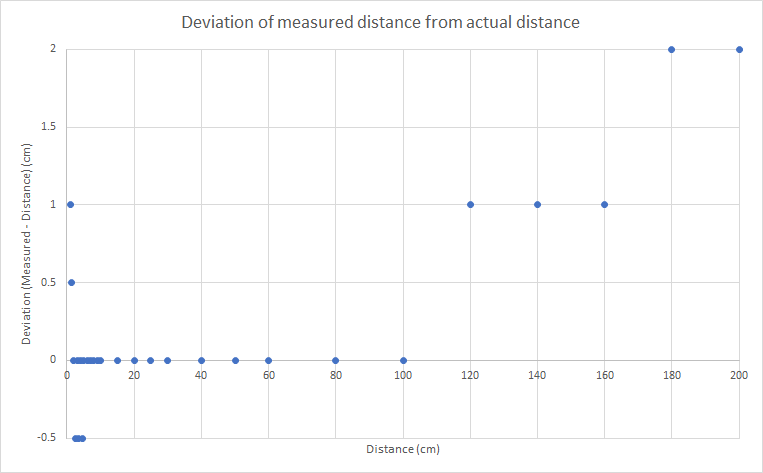
\includegraphics[width=0.9\textwidth]{ranger-measurement}
	\end{figure}

	The above chart shows the deviation from the actual distance as measured with the ultrasonic ranger by pointing it at a perpendicular wall certain distances away. The measurements for distances under $\SI{3}{cm}$ are all exactly $\SI{3}{cm}$, which explains the linearly decreasing distances in the lower end; as mentioned previously, the ranger cannot measure distances any closer. As distance increases, the measurement becomes less accurate: this may be because the father the pulse has to travel, the more spread out it becomes, and it bounces off parts of the wall not exactly perpendicular but slightly off centre. This explanation is further supported by the fact that when using a portable smaller surface in lieu of a wall, as I had originally done, at certain distances the surface wasn't large enough to yield a meaningful result.
\end{document}